\tikzset{every picture/.style={line width=0.75pt}} %set default line width to 0.75pt        
\begin{figure}[H]
\caption{Grafo di Overlap}
\begin{center}
Read: \texttt{ACGTGTG}, \texttt{CGTGTGC}, \texttt{GTGCCA}, \texttt{CCACG}
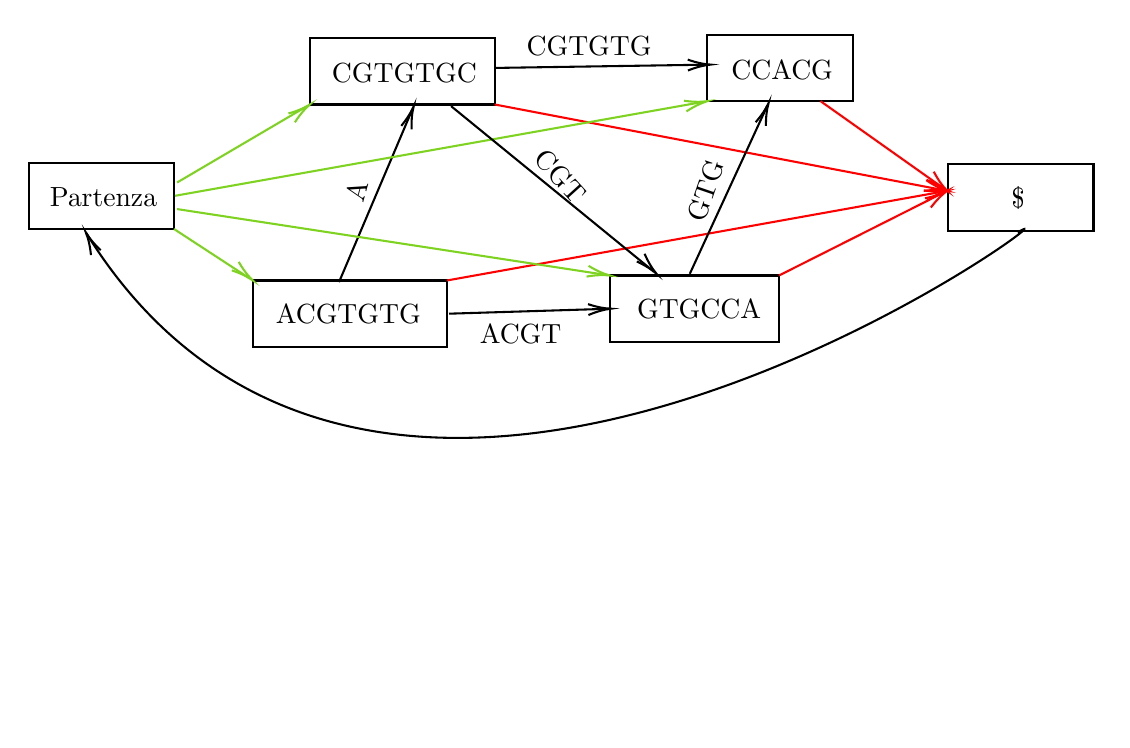
\begin{tikzpicture}[x=0.75pt,y=0.6pt,yscale=-1,xscale=1]
%uncomment if require: \path (0,281); %set diagram left start at 0, and has height of 281
%Shape: Rectangle [id:dp6560992130069507] 
\draw   (158.5,30) -- (247.5,30) -- (247.5,70) -- (158.5,70) -- cycle ;
%Shape: Rectangle [id:dp8633094909301302] 
\draw   (350,28) -- (420,28) -- (420,68) -- (350,68) -- cycle ;
%Straight Lines [id:da17421981355945193] 
\draw    (247.5,48) -- (349.5,46.04) ;
\draw [shift={(351.5,46)}, rotate = 538.9] [color={rgb, 255:red, 0; green, 0; blue, 0 }  ][line width=0.75]    (10.93,-3.29) .. controls (6.95,-1.4) and (3.31,-0.3) .. (0,0) .. controls (3.31,0.3) and (6.95,1.4) .. (10.93,3.29)   ;

%Shape: Rectangle [id:dp26552417711503384] 
\draw   (131,176) -- (224.5,176) -- (224.5,216) -- (131,216) -- cycle ;
%Shape: Rectangle [id:dp10524493499981546] 
\draw   (303,173) -- (384.5,173) -- (384.5,213) -- (303,213) -- cycle ;
%Straight Lines [id:da8474295750375322] 
\draw    (172.5,177) -- (207.86,72.89) ;
\draw [shift={(208.5,71)}, rotate = 468.76] [color={rgb, 255:red, 0; green, 0; blue, 0 }  ][line width=0.75]    (10.93,-3.29) .. controls (6.95,-1.4) and (3.31,-0.3) .. (0,0) .. controls (3.31,0.3) and (6.95,1.4) .. (10.93,3.29)   ;

%Straight Lines [id:da7595524463463148] 
\draw    (225.5,196) -- (301.5,193.08) ;
\draw [shift={(303.5,193)}, rotate = 537.8] [color={rgb, 255:red, 0; green, 0; blue, 0 }  ][line width=0.75]    (10.93,-3.29) .. controls (6.95,-1.4) and (3.31,-0.3) .. (0,0) .. controls (3.31,0.3) and (6.95,1.4) .. (10.93,3.29)   ;

%Shape: Rectangle [id:dp375619585347468] 
\draw   (466,106) -- (536,106) -- (536,146) -- (466,146) -- cycle ;
%Straight Lines [id:da8048124855752778] 
\draw [color={rgb, 255:red, 255; green, 0; blue, 0 }  ,draw opacity=1 ]   (404.5,68) -- (464,120.67) ;
\draw [shift={(465.5,122)}, rotate = 221.52] [color={rgb, 255:red, 255; green, 0; blue, 0 }  ,draw opacity=1 ][line width=0.75]    (10.93,-3.29) .. controls (6.95,-1.4) and (3.31,-0.3) .. (0,0) .. controls (3.31,0.3) and (6.95,1.4) .. (10.93,3.29)   ;

%Straight Lines [id:da91205814003782] 
\draw [color={rgb, 255:red, 255; green, 0; blue, 0 }  ,draw opacity=1 ]   (384.5,173) -- (463.81,123.07) ;
\draw [shift={(465.5,122)}, rotate = 507.8] [color={rgb, 255:red, 255; green, 0; blue, 0 }  ,draw opacity=1 ][line width=0.75]    (10.93,-3.29) .. controls (6.95,-1.4) and (3.31,-0.3) .. (0,0) .. controls (3.31,0.3) and (6.95,1.4) .. (10.93,3.29)   ;

%Straight Lines [id:da9132525115334023] 
\draw [color={rgb, 255:red, 255; green, 0; blue, 0 }  ,draw opacity=1 ]   (224.5,176) -- (463.55,122.44) ;
\draw [shift={(465.5,122)}, rotate = 527.37] [color={rgb, 255:red, 255; green, 0; blue, 0 }  ,draw opacity=1 ][line width=0.75]    (10.93,-3.29) .. controls (6.95,-1.4) and (3.31,-0.3) .. (0,0) .. controls (3.31,0.3) and (6.95,1.4) .. (10.93,3.29)   ;

%Straight Lines [id:da7445332124936079] 
\draw [color={rgb, 255:red, 255; green, 0; blue, 0 }  ,draw opacity=1 ]   (247.5,70) -- (463.55,121.54) ;
\draw [shift={(465.5,122)}, rotate = 193.42] [color={rgb, 255:red, 255; green, 0; blue, 0 }  ,draw opacity=1 ][line width=0.75]    (10.93,-3.29) .. controls (6.95,-1.4) and (3.31,-0.3) .. (0,0) .. controls (3.31,0.3) and (6.95,1.4) .. (10.93,3.29)   ;

%Curve Lines [id:da5406375819342921] 
\draw    (499.5,147) .. controls (539.5,117) and (195.5,440) .. (50.5,147) ;
\draw [shift={(50.5,147)}, rotate = 423.66999999999996] [color={rgb, 255:red, 0; green, 0; blue, 0 }  ][line width=0.75]    (10.93,-3.29) .. controls (6.95,-1.4) and (3.31,-0.3) .. (0,0) .. controls (3.31,0.3) and (6.95,1.4) .. (10.93,3.29)   ;

%Shape: Rectangle [id:dp7097560349466829] 
\draw   (23,105) -- (93,105) -- (93,145) -- (23,145) -- cycle ;
%Straight Lines [id:da08262697801168883] 
\draw [color={rgb, 255:red, 126; green, 211; blue, 33 }  ,draw opacity=1 ]   (94.5,117) -- (156.89,71.18) ;
\draw [shift={(158.5,70)}, rotate = 503.71] [color={rgb, 255:red, 126; green, 211; blue, 33 }  ,draw opacity=1 ][line width=0.75]    (10.93,-3.29) .. controls (6.95,-1.4) and (3.31,-0.3) .. (0,0) .. controls (3.31,0.3) and (6.95,1.4) .. (10.93,3.29)   ;

%Straight Lines [id:da5925934520006846] 
\draw [color={rgb, 255:red, 126; green, 211; blue, 33 }  ,draw opacity=1 ]   (93.5,125) -- (348.05,68.43) ;
\draw [shift={(350,68)}, rotate = 527.47] [color={rgb, 255:red, 126; green, 211; blue, 33 }  ,draw opacity=1 ][line width=0.75]    (10.93,-3.29) .. controls (6.95,-1.4) and (3.31,-0.3) .. (0,0) .. controls (3.31,0.3) and (6.95,1.4) .. (10.93,3.29)   ;

%Straight Lines [id:da9161535456154222] 
\draw [color={rgb, 255:red, 126; green, 211; blue, 33 }  ,draw opacity=1 ]   (94.5,133) -- (301.04,172.62) ;
\draw [shift={(303,173)}, rotate = 190.86] [color={rgb, 255:red, 126; green, 211; blue, 33 }  ,draw opacity=1 ][line width=0.75]    (10.93,-3.29) .. controls (6.95,-1.4) and (3.31,-0.3) .. (0,0) .. controls (3.31,0.3) and (6.95,1.4) .. (10.93,3.29)   ;

%Straight Lines [id:da5498196959860426] 
\draw [color={rgb, 255:red, 126; green, 211; blue, 33 }  ,draw opacity=1 ]   (93,145) -- (129.45,174.74) ;
\draw [shift={(131,176)}, rotate = 219.21] [color={rgb, 255:red, 126; green, 211; blue, 33 }  ,draw opacity=1 ][line width=0.75]    (10.93,-3.29) .. controls (6.95,-1.4) and (3.31,-0.3) .. (0,0) .. controls (3.31,0.3) and (6.95,1.4) .. (10.93,3.29)   ;

%Straight Lines [id:da4597957524218963] 
\draw    (226.5,71) -- (324.1,170.57) ;
\draw [shift={(325.5,172)}, rotate = 225.57] [color={rgb, 255:red, 0; green, 0; blue, 0 }  ][line width=0.75]    (10.93,-3.29) .. controls (6.95,-1.4) and (3.31,-0.3) .. (0,0) .. controls (3.31,0.3) and (6.95,1.4) .. (10.93,3.29)   ;

%Straight Lines [id:da11466253953137451] 
\draw    (341.5,172) -- (378.81,70.88) ;
\draw [shift={(379.5,69)}, rotate = 470.25] [color={rgb, 255:red, 0; green, 0; blue, 0 }  ][line width=0.75]    (10.93,-3.29) .. controls (6.95,-1.4) and (3.31,-0.3) .. (0,0) .. controls (3.31,0.3) and (6.95,1.4) .. (10.93,3.29)   ;


% Text Node
\draw (204,51) node  [align=left] {CGTGTGC};
% Text Node
\draw (386,49) node  [align=left] {CCACG};
% Text Node
\draw (177,196) node  [align=left] {ACGTGTG};
% Text Node
\draw (346,193) node  [align=left] {GTGCCA};
% Text Node
\draw (500,126) node  [align=left] {\$};
% Text Node
\draw (59,126) node  [align=left] {Partenza};
% Text Node
\draw (181,122) node [rotate=-285.42] [align=left] {A};
% Text Node
\draw (349,122) node [rotate=-288.92] [align=left] {GTG};
% Text Node
\draw (293,35) node  [align=left] {CGTGTG};
% Text Node
\draw (260,208) node  [align=left] {ACGT};
% Text Node
\draw (279,113) node [rotate=-47.91] [align=left] {CGT};
\end{tikzpicture}
\end{center}
\end{figure}